% Robocode AI Beamer Presentation (modeled after presentation_example.tex)
\documentclass[12pt,aspectratio=169]{beamer}

% THEME & COLORS
\usetheme{Madrid}
\setbeamertemplate{navigation symbols}{}
\setbeamertemplate{footline}[frame number]

\definecolor{mublue}{RGB}{0,51,102}
\definecolor{mugold}{RGB}{255,204,0}
\definecolor{codegray}{rgb}{0.95,0.95,0.95}
\definecolor{lightblue}{RGB}{228,240,252}

\usecolortheme[named=mublue]{structure}

\setbeamercolor{title}{fg=white,bg=mublue}
\setbeamercolor{frametitle}{fg=white,bg=mublue}
\setbeamercolor{block title}{fg=white,bg=mublue}
\setbeamercolor{block body}{bg=codegray}
\setbeamertemplate{blocks}[rounded][shadow=true]

% PACKAGES
\usepackage[utf8]{inputenc}
\usepackage{graphicx}
\usepackage{xcolor}
\usepackage{listings}
\usepackage{tikz}
\usetikzlibrary{arrows.meta,positioning,shapes.geometric,calc}

% CODE STYLE
\lstdefinestyle{pycode}{
  language=Python,
  basicstyle=\ttfamily\small,
  keywordstyle=\color{mublue}\bfseries,
  commentstyle=\color{gray},
  stringstyle=\color{teal},
  showstringspaces=false,
  breaklines=true,
  frame=single,
  backgroundcolor=\color{codegray}
}

% FONT TWEAKS
\setbeamerfont{frametitle}{size=\Large}
\setbeamerfont{title}{size=\LARGE}
\setbeamerfont{subtitle}{size=\large}
\setbeamerfont{normal text}{size=\large}
\setbeamerfont{itemize/enumerate body}{size=\large}
\setbeamerfont{itemize/enumerate subbody}{size=\normalsize}

% TITLE INFO
\title[Robocode DQN]{AI in Robocode}
\subtitle{DQN Bot Architecture and Training (Jacob3\_0)}
\author{Jacob Becker}
\institute{Misericordia University}

% DOCUMENT
\begin{document}

% TITLE SLIDE
{
  \setbeamertemplate{footline}{}
  \begin{frame}[plain]
    \centering
    \vspace{0.30cm}
    {\color{mublue}\Huge\textbf{\inserttitle}}\\[0.15cm]
    {\color{black}\textbf{\insertsubtitle}}\\[0.25cm]
    {\large\textbf{\insertauthor}}\\
    \insertinstitute\\[0.35cm]
  \end{frame}
}

%----------------1-----------------
\begin{frame}{Objectives}
  \begin{enumerate}
    \item Define the state space used by the bot
    \item Define the action space
    \item Explain DQN as a value-based RL method
    \item Show the objective function and training mechanics
    \item Show how performance will be measured
  \end{enumerate}
\end{frame}

%----------------2-----------------
\begin{frame}{Bot Architecture (Single Process)}
\centering
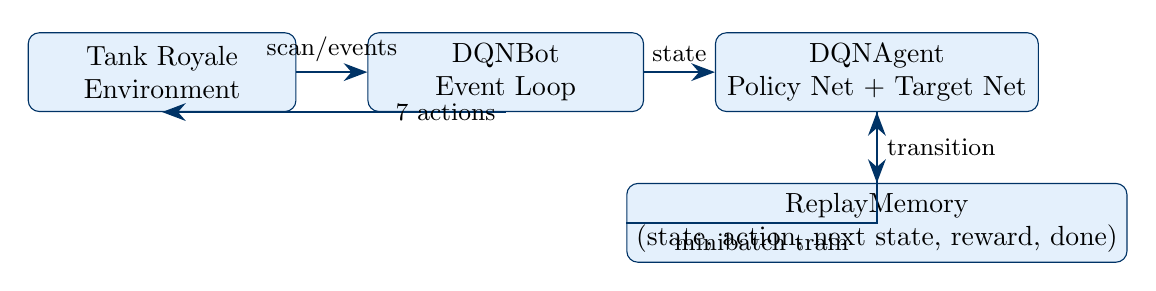
\begin{tikzpicture}[
  node distance=0.9cm and 0.9cm,
  box/.style={draw=mublue, rounded corners, fill=lightblue, minimum height=1.0cm, align=center, font=\normalsize},
  arrow/.style={-{Stealth[length=3mm]}, thick, draw=mublue}
]
\node[box, minimum width=3.4cm] (env) {Tank Royale\\Environment};
\node[box, right=of env, minimum width=3.5cm] (bot) {DQNBot\\Event Loop};
\node[box, right=of bot, minimum width=4.1cm] (agent) {DQNAgent\\Policy Net + Target Net};
\node[box, below=of agent, minimum width=4.1cm] (replay) {ReplayMemory\\(state, action, next state, reward, done)};
\draw[arrow] (env) -- node[above, font=\small] {scan/events} (bot);
\draw[arrow] (bot) -- node[above, font=\small] {state} (agent);
\draw[arrow] (agent) -- node[right, font=\small] {transition} (replay);
\draw[arrow] (replay.west) -| node[pos=0.27, below, font=\small] {minibatch train} (agent.south);
\draw[arrow] (bot.south) |- node[pos=0.2, left, font=\small] {7 actions} (env.south);
\end{tikzpicture}
\end{frame}

%----------------3-----------------
\begin{frame}{State Definition (16 Features)}
\begin{itemize}
  \item Self: normalized energy, speed, heading as $\sin/\cos$
  \item Position: normalized $x,y$ and distances to four walls
  \item Enemy: bearing as $\sin/\cos$, normalized distance, enemy energy
  \item Temporal: $\Delta$bearing and $\Delta$distance
  \item Weapon readiness: normalized gun heat
  \item Freshness: 1 if enemy scanned recently, else 0
\end{itemize}

\[
s_t \in \mathbb{R}^{16}
\]
\end{frame}

%----------------4-----------------
\begin{frame}{Action Definition (7 Discrete Actions)}
\begin{columns}[T,totalwidth=\textwidth]
\column{0.56\textwidth}
\begin{itemize}
  \item 0: strafe left
  \item 1: strafe right
  \item 2: forward
  \item 3: backward
  \item 4: fire power 1.0
  \item 5: fire power 2.0
  \item 6: fire power 3.0
\end{itemize}

\column{0.44\textwidth}
\[
a_t \in \{0,1,2,3,4,5,6\}
\]
\vspace{0.1cm}
\begin{block}{Reward signals in code}
Bullet hit: positive\\
Hit by bullet: negative\\
Wall hit: negative\\
Terminal win/loss: $+1/-1$
\end{block}
\end{columns}
\end{frame}

%----------------5-----------------
\begin{frame}{How DQN Works (Value-Based)}
\begin{itemize}
  \item Network predicts $Q_\theta(s,a)$ for all actions.
  \item Policy uses epsilon-greedy exploration.
  \item Exploit step picks action with maximum predicted value.
\end{itemize}

\[
\pi(s_t)=\arg\max_a Q_\theta(s_t,a)
\]

\[
\epsilon_t=\epsilon_{\min}+\left(\epsilon_{\max}-\epsilon_{\min}\right)\exp\left(-\frac{\text{steps}}{\text{decay}}\right)
\]

\begin{itemize}
  \item Jacob3\_0 network: MLP $16 \rightarrow 128 \rightarrow 128 \rightarrow 7$.
\end{itemize}
\end{frame}

%----------------6-----------------
\begin{frame}{Target, Loss, and Soft Update}
\begin{itemize}
  \item Mini-batches sampled from replay memory.
  \item Terminal transitions have zero next-state bootstrap value.
\end{itemize}

\[
y_t = r_t + \gamma (1-d_t) \max_{a'} Q_{\bar\theta}(s_{t+1},a')
\]

\[
\mathcal{L}(\theta)=\mathbb{E}\left[\operatorname{SmoothL1}\left(Q_\theta(s_t,a_t),y_t\right)\right]
\]

\[
\bar\theta \leftarrow \tau\,\theta + (1-\tau)\,\bar\theta
\]

\begin{itemize}
  \item Jacob3\_0 uses Adam, gradient clipping, and $\tau=0.005$.
\end{itemize}
\end{frame}

%----------------7-----------------
\begin{frame}[fragile]{Training Loop Snapshot}
\begin{lstlisting}[style=pycode]
state = self._encode_state()
action = self.agent.select_action(state)

if self.prev_state is not None:
    self.agent.push_transition(
        self.prev_state,
        self.prev_action,
        state,
        self.step_reward,
        done=False,
    )

self._execute_action(action)
\end{lstlisting}
\end{frame}

%----------------8-----------------
\begin{frame}{Performance Section (Fill In After Runs)}
\begin{block}{Metrics to report}
Win rate, average episode reward, steps survived, wall-hit count, reward variance.
\end{block}

\vspace{0.2cm}
\begin{itemize}
  \item Use the JSONL log file from training runs.
  \item Plot win rate and reward versus episode index.
  \item Compare different hyperparameter settings on same opponents.
\end{itemize}

\[
\text{WinRate}(N)=\frac{\#\text{wins in first }N\text{ episodes}}{N}
\]
\end{frame}

%----------------9-----------------
\begin{frame}{Conclusion}
\begin{itemize}
  \item This version is a complete DQN-only bot pipeline.
  \item State and action definitions are fixed and implemented.
  \item Objective is value fitting with SmoothL1 + soft target updates.
  \item Next step is empirical tuning and filling the results slide.
\end{itemize}
\end{frame}

%----------------10----------------
\begin{frame}{Q\&A}
  \centering
  \Huge{\color{mublue}Questions?}\\[1em]
  \large Jacob Becker\\
  \normalsize CPS485 Robocode AI Project
\end{frame}

\end{document}
